\chapter{Implementación} \label{sec:implementation}
    La materialización del análisis y diseño detallado en las secciones anteriores lo conforma el conjunto software que se incluye en el CD distribuido con la presente memoria. No obstante, en este apartado se ha querido comentar ciertos aspectos relevantes, que por la dificultad presentada y/o por el papel clave dentro de la aplicación merecen mención especial.
    
    \section{Stack Tecnológico}
    En este apartado se ofrece un comentario sobre las principales decisiones tomadas acerca de las tecnologías empleadas en el desarrollo de la aplicación web.
    
    \subsection{Git}
    Como se comentó en la exposición de motivos, Git es una tecnología clave para el control de versiones, y desde el principio se puso el foco en ella. Aunque existen otras herramientas muy válidas, como Mercurial, la decisión fue seguir la tendencia global.
    
    Formalmente, Git es un sistema de control de versiones distribuido, permitiendo gestionar los cambios introducidos en un conjunto de ficheros, conocido como \emph{repositorio}, por un número arbitrario de personas. Sus principales características son:
    
    \begin{itemize}
    	\item[-] \textbf{Basado en instantáneas}. Otros sistemas de control de versiones tratan la información que almacenan como un conjunto de archivos más sus cambios a lo largo del tiempo, los incrementos. En cambio, Git piensa en sus datos más como una serie de instantáneas de un sistema de archivos en miniatura. Así, cada vez que se efectúa un \emph{commit} o se guarda el estado de un proyecto, Git toma una fotografía de cómo se están todos los archivos en ese momento y almacena una referencia a esa instantánea. Además, para ser eficiente, si los archivos no han cambiado no almacena el archivo nuevamente, sino un enlace al archivo idéntico anterior almacenado. En resumen, Git trata los datos que gestiona como una secuencia de capturas.
    	\item[-] \textbf{Trabajo en local}. Git es un sistema distribuido que permite que todos los implicados en un proyecto tengan en su máquina una copia completamente funcional del repositorio. Así, la mayoría de las operaciones necesitan sólo archivos y recursos locales para funcionar, siendo muy poco lo que no se puede hacer sin conexión a Internet. 
    	\item[-] \textbf{Integridad de la información}. Es casi imposible que algo varíe en los archivos gestionados por Git sin que el sistema lo detecte, dado que a todos estos archivos se les aplica la función \emph{hash} SHA-1, obteniendo como resultado una cadena de 40 caracteres hexadecimales. Esta cadena es luego usada en todo momento para referenciar el contenido usado para generarla.
    	\item[-] \textbf{Seguridad ante accidentes}. Con Git es muy difícil que, una vez realizado un \emph{commit}, se pierda el trabajo almacenado.
    \end{itemize}
    
    En el presente proyecto el uso del control de versiones con Git ha sido intensivo y fundamental. El repositorio del proyecto, alojado en GitHub, puede ser accedido \href{https://github.com/misrraimsp/firstmarket}{aquí}.
    
    \subsection{Java}
    Una de las primeras decisiones que se tuvo que tomar fue qué lenguaje de programación emplear para construir la aplicación web, ya que aunque en la especificación de la oferta del proyecto se establecía que este debiera ser PHP, a posteriori la libertad fue total. Esta no es una decisión trivial, ya que determina en gran medida el resto del stack tecnológico utilizado. Tras una exploración de las diferentes alternativas, y dado el background adquirido a lo largo del plan de estudios, la opción tomada fue Java. Es cierto que existen alternativas potentes en el mundo de la programación web, pero también lo es que Java ocupa una posición muy madura y asentada en la industria, con un entorno de recursos disponibles para el estudiante defícilmente superable, y con una perspectiva de futuro, como mínimo, estable. La decisión tomada primó profundidad antes que anchura, en el sentido de preferir aumentar y depurar las habilidades en Java antes de expandir a otros lenguajes. Por supuesto, esto es muy discutible, pero se creyó que era la opción correcta.
    
    Resaltar, además, que la versión utilizada ha sido Java 11, que en la actualidad es la más reciente que ofrece soporte a largo plazo (LTS, \emph{Long Term Support}).
    \\
    
    Java es un lenguaje que, como muchos otros, ha ido evolucionando con el tiempo, dando como resultado un conjunto de capacidades muy variado. En 2014, con la publicación de Java 8, el lenguaje experimentó una de las mayores expansiones, si no la mayor, de su historia. En ese momento se le introdujeron potentes capacidades de programación declarativa, como las \emph{Labmda Expressions} y la \emph{Stream API}, que, en cierto modo, han revolucionado la programación Java (véase, por ejemplo, el framework de desarrollo de aplicaciones web \href{http://sparkjava.com/}{Spark}, que sólo usa capacidades Java 8+)
    \\
    
    \begin{lstlisting}[language=Java,caption=Programación declarativa con Java,label=list:java_declarative]
    private Set<Long> getIdsByExcludedStatus(ProductStatus excludedStatus) {
    return bookRepository
    .findAll()
    .stream()
    .filter(book -> !book.getStatus().equals(excludedStatus))
    .map(Book::getId)
    .collect(Collectors.toSet())
    ;
    }
    \end{lstlisting}
    
    Como se ha comentado, una de las intenciones de usar la tecnología Java era precisamente profundizar en su conocimiento. Así, se ha aprovechado el desarrollo de la presente aplicación para estudiar estas capacidades declarativas, aplicándolas progresivamente. Como ejemplo, en el listado \ref{list:java_declarative} se muestra la implementación del método \emph{getIdsByExcludedStatus}, perteneciente a la clase \emph{BookServer}. Se puede apreciar la facilidad de lectura que el estilo declarativo proporciona, además de la potencia expresiva. 
    \\
    
    También es necesario comentar un par de librerías que merecen especial mención, por la relevancia que han tenido en el proyecto:
    
    \paragraph{Project Lombok}
    Aparte del nombre de una isla indonesia (como Java), Lombok es una librería Java destinada a aumentar la productividad. Se encarga de suprimir la necesidad de especificar cierto código repetitivo, como los constructores, los \emph{getters} y los \emph{setters}, o los \emph{equals} y los \emph{hashCode}. Así, como se muestra en el listado \ref{list:lombok_close}, a través de anotaciones se puede ahorrar una grandísima cantidad de código, que es generado por esta herramienta automáticamente antes de la compilación.
    \\
    
    \begin{lstlisting}[language=Java,caption=Clase \emph{Role} usando las anotaciones Lombok,label=list:lombok_close]
    package misrraimsp.uned.pfg.firstmarket.core.model;
    
    import lombok.Data;
    import lombok.EqualsAndHashCode;
    
    import javax.persistence.Entity;
    
    @Data
    @EqualsAndHashCode(callSuper = true)
    @Entity
    public class Role extends BasicEntity {
    
    	private String name;
    
    }
    \end{lstlisting}
    
    No obstante, en cualquier momento se puede efectuar un \emph{Delombok} y ver el código generado, como se muestra en el listado \ref{list:lombok_open}. Como se aprecia, la cantidad de código ahorrado es más que significativa.
    \\
    
    \begin{lstlisting}[language=Java,caption=Clase \emph{Role} tras efectuar un \emph{Delombok},label=list:lombok_open]
    package misrraimsp.uned.pfg.firstmarket.core.model;
    
    import javax.persistence.Entity;
    
    @Entity
    public class Role extends BasicEntity {
    
	    private String name;
	    
	    public Role() {
	    }
	    
	    public String getName() {
	    	return this.name;
	    }
	    
	    public void setName(String name) {
	    	this.name = name;
	    }
	    
	    public String toString() {
	    	return "Role(name=" + this.getName() + ")";
	    }
	    
	    public boolean equals(final Object o) {
		    if (o == this) return true;
		    if (!(o instanceof Role)) return false;
		    final Role other = (Role) o;
		    if (!other.canEqual((Object) this)) return false;
		    if (!super.equals(o)) return false;
		    final Object this$name = this.getName();
		    final Object other$name = other.getName();
		    if (this$name == null ? other$name != null : !this$name.equals(other$name)) return false;
		    return true;
	    }
	    
	    protected boolean canEqual(final Object other) {
	    	return other instanceof Role;
	    }
	    
	    public int hashCode() {
		    final int PRIME = 59;
		    int result = super.hashCode();
		    final Object $name = this.getName();
		    result = result * PRIME + ($name == null ? 43 : $name.hashCode());
		    return result;
	    }
    }
    \end{lstlisting}
    
    \paragraph{SLF4J - Logback}
    SLF4J (Simple Logging Facade for Java) es una API Java para tareas de registro que implementa el patrón de diseño \href{https://en.wikipedia.org/wiki/Facade_pattern}{\emph{facade}}, el cual permite desacoplar completamente el código de la aplicación de la tecnología específica de registro que subyaga bajo la fachada.
    
    Logback es la tecnología elegida que en el presente proyecto se conecta como backend de SLF4J. Se trata de una librería moderna, diseñada por el fundador de la famosa Log4j (Ceki Gülcü), y que pretende ser su sucesora.
    
    La configuración se encuentra en el fichero \emph{classpath: logback-spring.xml}, donde se detallan todos los aspectos relevantes, como el formato utilizado en los registros o la política de escritura y rotación de los ficheros de registro producidos.
    
    Esta es una de las funcionalidades añadidas al proyecto que, aún siendo muy humilde, ha tenido enorme impacto en la facilidad de desarrollo y mantenimiento. Es clave que desde fases tempranas se tenga un sistema de registro, el cual poder utilizar, por ejemplo, en las múltiples tareas de depuración que se deben llevar a cabo casi constantemente.
    \\
    
    Por último, un apunte acerca del entorno de desarrollo utilizado. Durante las primeras semanas se usó el mismo que en toda la carrera: Eclipse. Sin embargo, en el transcurso de una formación en Spring tomada en fases iniciales del proyecto, se entró en contacto con \textbf{IntelliJ IDEA}. Desde entonces ese fue el IDE empleado, destacándose su capacidad de aumentar la productividad y su facilidad de uso.
    
    \subsection{Apache Maven}
    En el mundo del desarrollo software una fase de especial importancia es aquella encargada de transformar todos los archivos de código fuente del proyecto en un paquete susceptible de ser distribuido, instalado y ejecutado en cualquier máquina. A esto se le conoce como el proceso de construcción del proyecto, y representa una tarea no trivial desde el momento en que el proyecto en sí adquiere cierta complejidad.
    
    Antiguamente, este proceso tenía que ser diseñado e implementado \emph{ad hoc}, de una manera específica para cada proyecto. Sin embargo, en la actualidad este proceso se encuentra altamente optimizado. En el caso del mundo Java las principales herramientas empleadas al efecto son Apache Maven y Gradle.
    
    En el presente proyecto se ha optado por utilizar Apache Maven. La justificación reside en que el punto de partida fue el total desconocimiento de este tipo de tecnologías, y al representar Gradle, aparentemente, una suerte de superconjunto o mejora sobre Apache Maven, se juzgó conveniente tomar a este último como puerta de entrada o primer escalón, teniendo en cuenta, además, que Apache Maven aún posee una profunda implantación en la industria y la documentación y recursos de todo tipo para su estudio es ingente.
    
    Apache Maven supuso una revolución en la forma de construir software en el mundo Java. Pero esta herramienta va más allá, siendo concebida como una utilidad de gestión y de comprensión de los proyectos software. Tal como se explica en su \href{https://maven.apache.org/what-is-maven.html}{web oficial}, sus principales objetivos son:
    
    \begin{itemize}
    	\item[-] Facilitar la construcción software.
    	\item[-] Homogeneizar el proceso de construcción software.
    	\item[-] Ofrecer un lenguaje común a la hora de obtener información sobre un proyecto, es decir, establecer una manera homogénea de \emph{definir} a un proyecto software.
    	\item[-] Incentivar buenas prácticas de desarrollo software.
    \end{itemize}
    
    Las características que han permitido a Apache Maven alcanzar estos objetivos descansan en gran medida en:
    
    \begin{itemize}
    	\item[-] \textbf{Convención sobre configuración}. Como también se comentará en la sección \ref{sec:spring}, este principio de diseño persigue que el desarrollador sólo deba especificar los aspectos no convencionales, confiando para el resto en la configuración por defecto ofrecida por Apache Maven. Como dichos valores por defecto normalmente son reflejo de buenas prácticas, más o menos consensuados por agentes expertos en la materia, automáticamente se está consiguiendo alinear el proyecto a dichas buenas prácticas, al tiempo de estarse facilitando el propio trabajo de construcción software. La adopción de Apache Maven de este paradigma se traduce en, entre otros muchas cosas, establecer una distribución de carpetas y ficheros estándar para el proyecto, o seguir determinadas convenciones a la hora de compilar el código fuente o ensamblar los paquetes.
    	\item[-] \textbf{Interfaz común}. Muy ligado con el aspecto anterior está el hecho de que Apache Maven ofrece un marco de trabajo o interfaz común para la construcción de proyectos software. Como ya se comentó, antes de la existencia de este tipo de herramientas el software se construía de una manera singular en cada proyecto. Con Apache Maven, sin embargo, se establece una manera estándar o canónica de hacerlo. Así, cuando un desarrollador aprecia que un determinado proyecto está gestionado con Apache Maven puede asumir mucha información sobre él.
    	\item[-] \textbf{Reutilización a través de \emph{plugins}}. Apache Maven está diseñado de forma que se maximiza la flexibilidad y la reutilización de la lógica de construcción. El núcleo de la herramienta se encarga de muy pocas tareas, actuando más como un orquestador que lee la información centralizada acerca del proyecto en un fichero XML y delega el grueso del trabajo en plugins. Es decir, son los plugins los que realizan las diferentes labores de construcción, como compilar, instalar o empaquetar. Apache Maven ofrece una serie de plugins por defecto, pero también la posibilidad de construir nuevos e implementar la lógica de construcción que se desee. De hecho, en el presente proyecto se ha añadido el plugin que ofrece Spring Boot.
    	\item[-] \textbf{Modelo conceptual de proyecto}. Dicho lo anterior, la gran característica que aporta Apache Maven es la abstracción de toda la información necesaria referente a un proyecto en un fichero, el \textbf{Project Object Model} (en el presente proyecto ver el fichero \emph{pom.xml}). En él se especifica, entre otras cosas, las dependencias con otros proyectos, de forma que es Apache Maven quien se encarga de gestionarlas, esto es, resolverlas, descargarlas de un repositorio central, colocarlas en las carpetas apropiadas, enlazarlas durante la construcción, etc. En el listado \ref{list:maven_dependency} se muestra, como ejemplo, la declaración de una dependencia con la librería \href{https://www.passay.org/}{Passay}, utilizada en la aplicación web para generar nuevas contraseñas aleatorias. 
    \end{itemize}
    
    \begin{lstlisting}[caption=Declaración de dependencia en Apache Maven, label=list:maven_dependency]
    <dependency>
    <groupId>org.passay</groupId>
    <artifactId>passay</artifactId>
    <version>1.5.0</version>
    </dependency>
    \end{lstlisting}
    
    El desarrollo del presente proyecto ha servido para tomar un primer contacto serio con Apache Maven, resultando de vital importancia para la construcción y para la gestión de dependencias.
    
    \subsection{Spring} \label{sec:spring}
    Sin duda, Spring ha sido una de las tecnologías que más impacto ha tenido en el presente proyecto. En esta sección se pretende dar una idea lo más general y amplia posible de sus características.
    
    Lo primero a aclarar es qué se entiende por \emph{Spring}, ya que su significado puede variar dependiendo del contexto. Puede que se refiera en concreto al proyecto \emph{Spring Framework}, donde empezó todo allá por el año 2003, o al ecosistema completo formado por todos los \href{https://spring.io/projects}{proyectos Spring}, esto es, por Spring Framework más todos los otros proyectos Spring que se desarrollaron posteriormente utilizando como núcleo al primero.
    
    Los proyectos Spring usados en el desarrollo de la aplicación web han sido \emph{Spring Framework}, \emph{Spring Boot}, \emph{Spring Data JPA} y \emph{Spring Security}. En la presente sección se dará una descripción de las principales características de cada uno de ellos que han tenido relación con el desarrollo del presente proyecto, salvo aquellas referentes a Spring Security, tratadas por separado en la sección \ref{sec:springsec} en el marco de la seguridad de la aplicación web.
    
    \paragraph{Spring Framework} 
    En este apartado se esbozará las principales características de esta parte fundamental dentro del ecosistema Spring, tomando para ello como principal fuente su propia \href{https://docs.spring.io/spring/docs/current/spring-framework-reference/}{documentación}.
    
    Tal como establecen sus autores, los principios de diseño que han guiado su desarrollo a lo largo del tiempo han sido:
    
    \begin{itemize}
    	\item[-] Estar orientado a permitir que se tomen las decisiones de diseño lo más tarde posible. Por ejemplo, permite cambiar la tecnología de persistencia sin alterar el código de la aplicación (esto fue constatado en el desarrollo de la aplicación web, al pasar de forma transparente, en una etapa bastante avanzada del proyecto, de MariaDB a PostgreSQL).
    	\item[-] Ser capaz de acomodar diferentes perspectivas de desarrollo. Spring es extensamente configurable, no imponiendo ningún estilo o manera de resolver los problemas.
    	\item[-] Ser altamente retrocompatible.
    	\item[-] Tomar muchas precauciones a la hora de diseñar las APIs, de forma que sean intuitivas y perduren a través de las diferentes versiones.
    	\item[-] Seguir los más altos estándares de calidad del código.
    \end{itemize}
    
    De todas las funcionalidades integradas dentro del proyecto Spring Framework, la más importante es el contenedor de Inversión de Control (inversion of control, IoC). Este concepto, tratado en la sección \ref{sec:ioc}, hace referencia a la capacidad de gestionar el ciclo de vida de los \emph{beans}, que es como en el ecosistema Spring se conoce a los objetos gestionados por el contenedor.
    
    La interfaz \emph{org.springframework.context.ApplicationContext}, que representa el contenedor de IoC de Spring, es la responsable de instanciar, configurar y ensamblar los \emph{beans}.
    
    Por su parte, el contenedor conoce qué objetos instanciar y cómo configurarlos y ensamblarlos entre sí a través de la lectura de metadatos de configuración especificados por el desarrollador.
    
    La figura \ref{fig:container_magic}, tomada de la documentación oficial, muestra un diagrama de alto nivel de cómo funciona lo explicado. Esto es, el código desarrollado en forma de POJOs (Plain Old Java Object) es gestionado en el contenedor de IoC según se haya especificado en los metadatos de configuración, produciendo como resultado una aplicación completamente funcional.
    
    \begin{figure}[hbt!]
    	\centering
    	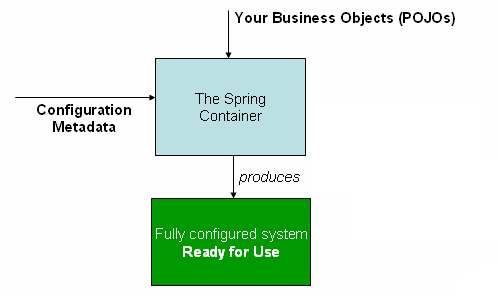
\includegraphics[width=0.8\textwidth,keepaspectratio]{container_magic}
    	\caption{Flujo de información en el contenedor de IoC}
    	\label{fig:container_magic}
    \end{figure}
    
    Existen diversas formas de especificar los metadatos de configuración. La manera original fue a través de un fichero XML, pero en la actualidad también se puede realizar con anotaciones insertadas en el código de la aplicación (añadido en la versión 2.5), o con código Java dedicado de configuración (añadido en la versión 3.0). El contenedor de IoC está completamente desacoplado de estos mecanismos de especificación de los metadatos de configuración.
    
    Existe la cuestión de qué tipo de configuración es mejor. La respuesta no es clara, ya que cada opción posee su dosis de ventajas e inconvenientes. Las anotaciones son la manera más concisa y quizás mas simple para un principiante, pero mezclan código de negocio con configuración del framework, algo que mina el principio de separación de responsabilidades. Además poseen el inconveniente de descentralizar la configuración, impactando negativamente en su mantenibilidad. La configuración con código Java permite un control centralizado, pero se pierde en facilidad y brevedad. Por su parte, los ficheros XML son inmejorables a la hora separar responsabilidades, pudiéndose alterar la configuración sin tocar una línea de código y, por tanto, sin tener que recompilar. El inconveniente de este sistema es el elevado tamaño y complejidad que muchas veces estos ficheros alcanzan, siendo además su curva de aprendizaje más pronunciada.
    
    En el desarrollo de la presente aplicación web se ha utilizado la configuración a través de anotaciones y de código Java dedicado. Además, se ha utilizado Spring Boot, lo que, como se verá, implica que una gran parte (la mayoría) de la configuración necesaria ha sido establecida por defecto.
    \\
    
    Además del contenedor de IoC, la aplicación web desarrollada hace uso de otras capacidades ofrecidas por Spring Framework:
    
    \begin{itemize}
    	\item[-] Publicación y escucha de eventos.
    	\item[-] Gestión de transacciones.
    	\item[-] Planificación de tareas.
    	\item[-] Validación.
    	\item[-] El framework de desarrollo web \emph{Spring Web MVC} (comúnmente conocido como simplemente Spring MVC).
    \end{itemize}
    
    Spring MVC, como muchos otros frameworks de desarrollo web, está implementado alineado con el patrón de diseño \emph{Front Controller}, donde un Servlet central, el llamado \emph{DispatcherServlet}, recibe las peticiones HTTP y delega su procesamiento a los componentes apropiados, en el caso de la presente aplicación los objetos anotados con \emph{@Controller}. Cada uno de estos objetos es responsable de llevar a cabo las acciones necesarias para cada \emph{endpoint} expuesto, apoyándose para ello en la capa de negocio, es decir, en los objetos anotados con \emph{@Service}. Como ya se explicó en la sección \ref{sec:design_layer}, estos objetos \emph{@Service} se apoyan, a su vez, en otros objetos de su clase y en objetos anotados con \emph{@Repository}, que actúan como puerta de entrada a los datos. Cumplida la lógica de negocio, el objeto \emph{@Controller} implicado devuelve el nombre de la vista a proporcionar como respuesta, así como los datos con los que poblarla. El motor de plantillas genera en este punto el contenido HTML, que es devuelto por el \emph{DispatcherServlet} al usuario.
    
    En resumen, Spring MVC ofrece la infraestructura \emph{Front Controller}, esto es, los objetos necesarios para resolver el mapeo de las peticiones HTTP a los métodos apropiados de los objetos \emph{@Controller}, los objetos encargados de resolver las vistas, los encargados del enlace de datos, etc, permitiendo al desarrollador centrarse en especificar la lógica de negocio.
    
    \paragraph{Spring Boot}
    Este proyecto ha sido el gran avance de los últimos años dentro del universo Spring. De hecho, ha cambiado por completo el paradigma, permitiendo el desarrollo de aplicaciones totalmente funcionales en un espacio de tiempo dramáticamente inferior al necesario con anterioridad a su aparición. Tal como viene recogido en la \href{https://docs.spring.io/spring-boot/docs/current-SNAPSHOT/reference/html/}{documentación} oficial, sus principales objetivos son:
    
    \begin{itemize}
    	\item[-] Ofrecer una vía de entrada al uso de las tecnologías Spring radicalmente más rápida y sencilla.
    	\item[-] Proporcionar una configuración por defecto sensata, y al mismo tiempo de ágil modificación si los requisitos así lo necesitan.
    	\item[-] Ofrecer todo un abanico de funcionalidades transversales a la mayoría de aplicaciones, como los servidores embebidos.
    	\item[-] Supresión de la necesidad de configuración a través de ficheros XML.
    \end{itemize}
    
    Así, Spring Boot no es una alternativa a otros proyectos Spring. Su objetivo no es proporcionar nuevas soluciones para problemas ya resueltos, sino ofrecer una manera de mejorar el aprovechamiento del ecosistema entero, fomentando una experiencia de desarrollo que simplifique el uso de los módulos ya disponibles. Esto hace que Spring Boot sea una opción ideal para toda clase de desarrolladores, tanto los que ya están familiarizados con el ecosistema Spring como aquellos recién llegados, al permitirles adoptar las tecnologías de Spring de una manera simplificada. En este sentido, Spring Boot ha supuesto un vector de expansión de las tecnologías Spring, disminuyendo su barrera de entrada y maximizando el aprovechamiento de sus variadas funcionalidades.
    
    En gran medida, lo expuesto se consigue gracias a que Spring Boot ejercita el paradigma de diseño conocido como Convención sobre Configuración (\emph{Convention over Configuration, CoC}), o también como Código por Convención (\emph{Coding by Convention}). Este principio de diseño trata de disminuir el número de decisiones que el desarrollador debe tomar y aliviar así la complejidad de tener que configurar todas y cada una de las áreas que conforman una aplicación, todo ello sin necesariamente merma alguna en la flexibilidad. Así, el desarrollador sólo está llamado a especificar los aspectos no convencionales de la configuración de la aplicación, obteniendo como resultado inmediato un aumento en la productividad considerable.
    
    Conviene destacar también que Spring Boot permite ejecutar aplicaciones web sin necesidad de hacerlo en un contenedor de servlets externo o un servidor de aplicaciones, ya que el propio Spring Boot incluye un Tomcat embebido, el cual se despliega automáticamente en tiempo de ejecución.
    
    \paragraph{Spring Data JPA - Hibernate ORM}
    El proyecto Spring Data JPA, parte de la amplia familia Spring Data, es una capa de abstracción extra sobre la implementación de la especificación JPA que se utilice, que en el caso del presente proyecto ha sido Hibernate ORM.
    
    Por persistencia se hace referencia a la funcionalidad que permite que determinados objetos creados por la aplicación puedan sobrevivir más allá de la frontera de la misma. En términos Java, se trata de que el estado de ciertos objetos pueda perdurar fuera del entorno de la JVM, de modo que dicho estado esté disponible en cualquier momento posterior.
    
    \begin{figure}[hbt!]
    	\centering
    	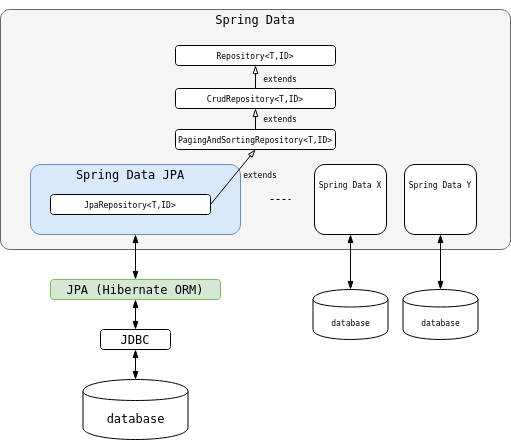
\includegraphics[width=\textwidth,keepaspectratio]{data_access}
    	\caption{Esquema de la infraestructura de acceso a datos}
    	\label{fig:data_access}
    \end{figure}
    
    JPA es una especificación que define una API de mapeo objeto-relacional y gestión de objetos persistentes. Además, hace innecesario el tratamiento explícito de las conexiones/recursos usuales al trabajar directamente con JDBC. Actualmente se encuentra en su versión 2.2, siendo su implementación de referencia EclipseLink. No obstante, Spring usa por defecto Hibernate ORM como proveedor de JPA, y en el presente proyecto no se ha modificado dicha configuración preestablecida.
    
    El mapeo objeto-relacional es la funcionalidad que permite la traducción entre los objetos de la aplicación (llamados entidades en este contexto) y las tablas de la base datos. Esto implica gestionar, entre otras cosas, las relaciones que existen entre las entidades. Esta es una tarea no trivial que los proyectos con necesidades de persistencia relacional (en contraposición con los modelos no relacionales, no tratados en el presente proyecto) deben afrontar. En este sentido, Hibernate ORM (Object/Relational Mapping) es un framework que permite la simplificación y en parte automatización de esta tarea. Como ejemplo, y sin entrar en detalles, las relaciones entre las entidades son especificadas a través de las anotaciones \emph{@OneToOne}, \emph{@OneToMany}, \emph{@ManyToOne} y \emph{@ManyToMany}.
    
    Resaltar que además del mapeo objeto-relacional, la abstracción JPA ofrece (de la mano de Hibernate ORM, en este caso) la gestión del ciclo de vida de las entidades y el lenguaje de consultas relacionales orientado a objeto JPQL. En el listado \ref{list:jpql} se muestra un ejemplo de consulta con este lenguaje extraído del presente proyecto.
    
    \begin{lstlisting}[caption=Ejemplo de consulta especificada en JPQL,label=list:jpql]
    @Query("SELECT b.id FROM Book b WHERE b.publisher.id IN :publisherIds")
    Set<Long> findIdByPublisherIds(@Param("publisherIds") Set<Long> publisherIds);
    \end{lstlisting}
    
    En este punto, vistas las capacidades de abstracción que ofrece JPA a través de sus implementaciones, cabe preguntarse porqué añadir otra capa de abstracción encima con Spring Data JPA. La respuesta es que esta tecnología añade aún más facilidades de desarrollo y mantenimiento, en concreto:
    
    \begin{itemize}
    	\item[-] Permite la integración de JPA con el ecosistema Spring de una forma natural.
    	\item[-] Permite la adopción del patrón de diseño \emph{Repositorio} (ver sección \ref{sec:design_layer}) sin necesidad de añadir código extra, ya que Spring Data JPA, como subconjunto de Spring Data, proporciona una serie de interfaces al efecto, tal como se esquematiza en la figura \ref{fig:data_access}. Así, construir una interfaz repositorio para cualquier entidad de la aplicación es tan fácil como extender alguna de las proporcionadas. En el presente proyecto todos los repositorios extienden a \emph{CrudRepository\textless{}T,ID\textgreater{}}.
    	\item[-] Además de ofrecer las interfaces, también lo hace con sus implementaciones. Es decir, el desarrollador puede olvidarse de crear código que implemente las interfaces de acceso a datos, Spring Data JPA lo realiza automáticamente.
    	\item[-] Posibilidad de inferir las consultas de acceso a datos a partir del nombre del método en la interfaz. Esta funcionalidad ha sido usada extensamente en el desarrollo del presente proyecto. En el listado \ref{list:query_inference} se muestra un método de la interfaz \emph{SecurityTokenRepository}, a partir del cual Spring Data JPA construye la consulta necesaria para obtener los \emph{SecurityToken} que cumplan estar asociados a un usuario determinado, con un \emph{SecurityEvent} dado y creados después de un punto temporal dado.
    \end{itemize}
    
    \begin{lstlisting}[caption=Ejemplo de método a partir del cual Spring Data JPA infiere la consulta apropiada,label=list:query_inference]
    Set<SecurityToken> findByTargetUserAndSecurityEventAndCreatedDateAfter(User targetUser, SecurityEvent securityEvent, LocalDateTime dateTime);
    \end{lstlisting}
    
    En resumen, Spring Data JPA añade una capa de abstracción sobre JPA, lo que significa que hace uso de todas las funcionalidades que esta especificación proporciona, y además suministra sus propias facilidades, como la implementación sin código del patrón \emph{Repositorio} o la creación de consultas a la base datos a partir del nombre de los métodos.
    
    \subsection{Thymeleaf} \label{sec:thymeleaf}
    Thymeleaf es un motor de plantillas para aplicaciones Java, tanto web como de escritorio, que permite crear dinámicamente documentos HTML5 (y otros, como XML o XHTML). Como principales características de esta tecnología cabe resaltar:
    
    \begin{itemize}
    	\item[-] Thymeleaf ejercita el concepto llamado \emph{natural templating}, esto es, las propias plantillas son documentos HTML5 válidos, de forma que prácticamente cualquier navegador las puede renderizar, mostrando su contenido por defecto. Esto es muy útil en la fase de desarrollo de la aplicación, ya que no hay necesidad de contar con un contenedor web para visualizar el resultado de la plantilla (como ocurre con la tecnología JSP), facilitando el trabajo paralelo sobre una misma vista en las labores frontend y backend.
    	\item[-] Es altamente extendible. Cualquiera puede crear su propio conjunto de atributos o etiquetas, con los nombres que se desee, definir sintaxis para expresiones y su lógica de evaluación, etc. Esto es, es posible crear lo que se denominan \emph{dialectos} de Thymeleaf, actuando así esta tecnología como un framework de plantillas. Por defecto se usa el conocido como dialecto \emph{Standard}.
    	\item[-] Thymeleaf se integra con muchísima facilidad con la tecnología Spring. De hecho, desde Spring se recomienda preferentemente su uso. Así, se dispone de un dialecto propio: el \emph{SpringStandard}, el cual permite el uso de Spring Expression Language. La integración con Spring Security es muy sencilla, permitiendo acoplar lógica de autenticación y/o autorización en las plantillas de una manera muy poco intrusiva.
    \end{itemize}
    
    En el presente proyecto, los documentos incorporados en \emph{classpath: resources/templates} son las plantillas HTML que el motor toma, junto con los datos de negocio que Spring MVC le suministra, para producir el contenido HTML5 que se sirve al cliente.
    
    \subsection{Bootstrap}
    En el ámbito del diseño frontend de la presente aplicación, la herramienta que más ha destacado a sido Bootstrap, versión 4. Se trata de un framework de HTML, CSS y JavaScript, que prima el desarrollo \emph{responsive}. Esto quiere decir que la aplicación web adapta su presentación al tamaño de la pantalla disponible, esto es, que \emph{responde} automáticamente a los cambios de tamaño de pantalla, de forma que en cada caso optimiza la presentación.
    
    Gracias a Bootstrap, con relativamente poco esfuerzo se puede ofrecer una experiencia de usuario muy correcta. Un gran número de elementos HTML como formularios, botones, encabezados, etc. son proporcionados por este framework, con estilo CSS ya preconfigurado, además de otros elementos como \emph{spinners}, \emph{modals}, \emph{cards} etc., lo que aumenta enormemente la productividad.  Además, aparte de los objetos, Bootstrap permite controlar el layout de las vistas de una manera muy sencilla y potente, basada en los Flexbox de CSS.
    
    Cuando el framework no es capaz de ofrecer una funcionalidad siempre se pueden usar directamente hojas de estilo CSS3, como ha sido el caso en el presente proyecto en varias ocasiones (\emph{classpath: resources/static/css/fmstyle.css}). Además, se han utilizado otros componentes que merecen especial mención:
    
    \begin{itemize}
    	\item[-] \href{https://fontawesome.com/}{FontAwesome}. Todos los iconos mostrados en la aplicación web han sido obtenidos de FontAwesome.
    	\item[-] \href{https://lokesh-coder.github.io/pretty-checkbox/}{Pretty Checkbox}. Con el objetivo de dar un mejor aspecto a los \emph{check boxes} utilizados, respecto del ofrecido por Bootstrap, se decidió usar esta librería CSS.
    	\item[-] \href{https://fonts.google.com/}{Google Fonts}. A efectos de dar un cariz más personalizado a la aplicación web se usó este servicio de Google. La fuente usada en la aplicación web ha sido \href{https://fonts.google.com/specimen/Noto+Serif+JP}{Noto Serif JP}.
    \end{itemize}
    
    \section[Pagos con Stripe]{Gestión de Pagos con Stripe} \label{sec:stripe}
    Los comercios, ya sean presenciales u \emph{online}, son en esencia lugares de intercambio. Normalmente, lo que una de las partes ofrece a la otra es dinero, a través de un pago. Por tanto, cabe esperar que, en cualquiera de estos establecimientos, el procedimiento por el cual se materializa el pago tome un lugar especial dentro de la lógica de negocio.
    
    Los comercios en Internet tienen, además, la responsabilidad de ofrecer altos estándares de seguridad a sus clientes, especialmente en lo concerniente con el pago. De hecho, una de las principales barreras que aparta a potenciales usuarios del comercio \emph{online} es la percepción de inseguridad que el proceso de pago telemático lleva asociado. En este sentido, el comercio a través de Internet depende de una manera radical en la confianza de los usuarios, siendo así este uno de los principales capitales a cultivar y fortalecer.
    
    La percepción de inseguridad no es en absoluto infundada. El notable desarrollo de la sociedad de la información a lo largo de las últimas décadas lleva inevitablemente asociado el incremento de las modalidades y de la capacidad de fraude digital. No obstante, en una pugna continua, la tecnología anti-fraude trata de mantenerse en todo momento actualizada para ejercer de contrapeso.
    
    Así, como se ha comentado, el pago es una tarea de vital importancia, transversal a todas las plataformas de comercio, con unos estrictos requisitos de seguridad a fin de generar la confianza que demanda el mercado. Es en este contexto donde juegan un papel esencial los proveedores de servicios de pago \emph{online}.
    
    Actualmente en el mercado existen múltiples alternativas de servicios de este tipo, como \href{https://www.paypal.com/}{PayPal} o \href{https://securionpay.com/}{SecurionPay}, pero el elegido para el desarrollo del presente proyecto ha sido \href{https://stripe.com/}{Stripe}. Amén de su consolidada posición en el mercado como uno de los servicios líderes en el sector, la principal característica diferenciadora ha sido la \href{https://stripe.com/docs}{cuidada colección} de documentación, guías, ejemplos, etc. que mantienen para facilitar la integración con su infraestructura. 
    
    \paragraph{Integración}
    Fundamentalmente, la aplicación web desarrollada se integra con la infraestructura de Stripe haciendo uso de dos puntos de enlace, uno en \emph{backend} y otro en \emph{frontend}:
    
    \begin{itemize}
    	\item[-] Una extensa interfaz de programación backend, \href{https://stripe.com/docs/api}{Stripe API}, para varios lenguajes (entre ellos Java), plena de funcionalidades que cubren multitud de casos de uso relacionados con la gestión de transacciones monetarias y sus aspectos asociados.
    	
    	La integración de la presente aplicación web se ha basado en el objeto \href{https://stripe.com/docs/api/payment_intents}{PaymentIntent}. Un PaymentIntent mantiene la información relacionada con un pago puntual. Entre dicha información, una pieza clave es el \emph{client\_secret}, que es el código identificativo de la transacción que permite al cliente, usándolo como parámetro en la invocación de funciones en \emph{Stripe.js}, finalizar el pago. Además, el PaymentIntent mantiene la información sobre la situación del pago que gestiona al recorrer una serie de \href{https://stripe.com/docs/payments/intents#intent-statuses}{estados} desde su creación (su ciclo de vida). Como se verá, FirstMarket conoce de estos estados al escuchar las notificaciones que Stripe le envía al \emph{webhook} configurado.
    	
    	\item[-] Una librería frontend, \href{https://stripe.com/docs/js}{\emph{Stripe.js}}, que permite, entre otras cosas, gestionar la comunicación entre el cliente y Stripe, y la inserción de elementos gráficos configurables en las vistas que la aplicación web sirve al cliente. Estos \href{https://stripe.com/docs/js/elements_object}{elementos} son empleados para recabar la información sensible de los formularios de pago (por ejemplo, el número de la tarjeta de débito).
    	
    	La presente aplicación web coordina todo el proceso de pago en el lado del cliente mediante el script desarrollado \emph{checkout.js}. En él, como se muestra en el listado \ref{list:js_checkout_card}, se ha usado el elemento \emph{card} ofrecido en \emph{Stripe.js}. En la figura \ref{fig:checkout_form} se muestra el resultado obtenido, siendo el citado elemento \emph{card} la entrada del formulario donde se solicita la información de la tarjeta bancaria.
    \end{itemize}
    
    \begin{lstlisting}[language=Javascript,caption=Extracto de checkout.js donde se crea y enlaza el elemento \emph{card},label=list:js_checkout_card]
    //...
    
    let stripe = Stripe(stripePublicKey);
    let elements = stripe.elements();
    let cardElement = elements.create('card');
    cardElement.mount('#card-element');
    
    //...
    \end{lstlisting}
    
    \begin{figure}[hbt!]
    	\centering
    	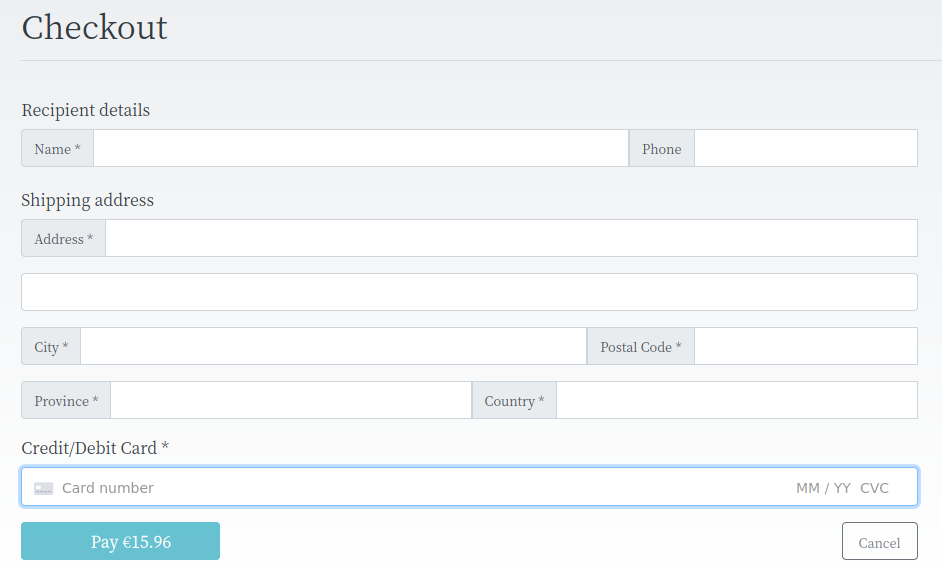
\includegraphics[width=\textwidth,keepaspectratio]{checkout_form}
    	\caption{Formulario de checkout}
    	\label{fig:checkout_form}
    \end{figure}
    
    \begin{figure}[hbt!]
    	\centering
    	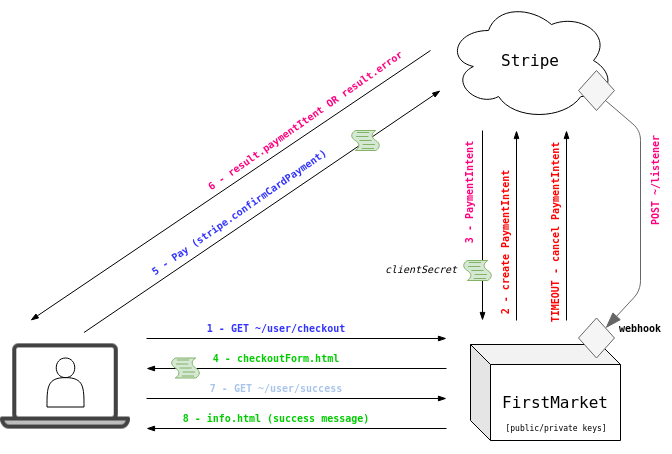
\includegraphics[width=\textwidth,keepaspectratio]{stripe}
    	\caption{Flujo de información durante un pago}
    	\label{fig:stripe}
    \end{figure}
    
    Una vez se ha comentado todo lo anterior, se está en disposición de esbozar el flujo de información que tiene lugar durante el proceso de pago, tomando como apoyo el esquema presentado en la figura \ref{fig:stripe}:
    
    \begin{itemize}
    	\item[1.] El cliente, estando en la vista de su cesta, decide proceder a finalizar la compra y hace click en el botón de ckeckout. Esto se traduce en una petición a FirstMarket al \emph{endpoint} GET \nolinkurl{~/user/checkout}. 
    	\item[2.] Tal como se explica en \ref{sec:concurrencia}, el sistema comprueba la disponibilidad de los libros pedidos y, si es el caso, compromete la cesta. En el proceso de comprometer la cesta contacta con Stripe para crear el PaymentIntent, especificando en este punto, entre otras cosas, la cantidad exacta a cobrar.
    	\item[3.] Stripe devuelve al sistema el PaymentIntent recién creado, el cual contiene el \emph{client\_secret}.
    	\item[4.] El sistema sirve la vista \emph{checkoutForm.html} al cliente, la cual lleva inserta el \emph{client\_secret}. Resaltar en este punto la importancia del encriptado que protocolos de transporte seguro proporcionan, ya que este código sólo debe ser conocido, fuera de Stripe y de Firstmarket, por el cliente. Así, como se explica en la sección \ref{sec:https}, la aplicación web desarrollada emplea HTTPS.
    	\item[5.] Tras completar correctamente el formulario de checkout (presentado en la figura \ref{fig:checkout_form}), el cliente presiona el botón de pagar. Esto desencadena que desde \emph{checkout.js} se invoque la función \emph{confirmCardPayment} (perteneciente a la librería \emph{Stripe.js}), tomando como parámetro, entre otros valores, el \emph{client\_secret}.
    	\item[6.] Stripe procesa el pago y responde al cliente enviándole el objeto \emph{result} (más adelante se explicará que en este punto, y en otros, Stripe notifica a FirstMarket a través del \emph{webhook}). Dependiendo del éxito o no del pago, este objeto contendrá en su interior, respectivamente, el PaymentIntent o un objeto \emph{error}. En ambos casos, \emph{checkout.js} toma las medidas oportunas. En caso de éxito, se realiza lo explicado en el siguiente punto. En caso contrario se notifica por pantalla al cliente para que tome las medidas oportunas.
    	\item[7.] \emph{checkout.js} realiza en background una petición a FirstMarket al \emph{endpoint} GET \nolinkurl{~/user/success}.
    	\item[8.] El sistema sirve la vista \emph{info.html} al cliente, la cual le comunica que el pedido se ha realizado con éxito y que pronto recibirá confirmación por email.
    \end{itemize}
    
    Notar en la figura \ref{fig:stripe} que, tal como se explicó en la sección \ref{sec:concurrencia}, cuando se produce el \emph{timeout} y el pago no se ha efectuado se activa la vía de descomprometer la cesta y, por tanto, cancelar el PaymentIntent.
    
    Por otro lado, podría pensarse que FirstMarket conoce de la finalización con éxito del pago a través de la solicitud que en el punto 7 anterior el cliente le realiza. Sin embargo, esa solicitud sólo es usada en backend como disparador para servir el mensaje estándar de finalización de una compra. Es decir, el sistema no realiza ninguna acción de lógica de negocio (no crea ningún pedido, de modifica ninguna cesta, etc.) al recibir la petición del punto 7. Sólo se limita a servir una vista con un mensaje. De hecho, cualquier cliente con sesión abierta en FirstMarket puede escribir en su navegador la dirección \nolinkurl{~/user/success} y el sistema le devolverá el mensaje de compra finalizada (por supuesto, sin haber realizado ninguna compra en realidad).
    
    Esto es así porque para conocer del estado de un pago FirstMarket no debe depender del cliente, sino de Stripe directamente. Y esta comunicación directa se realiza por medio del \emph{webhook} configurado en Stripe. Esto es, Stripe permite configurar el envío de notificaciones POST ante los eventos que se desee, existiendo multitud de \href{https://stripe.com/docs/api/events/types}{eventos disponibles}. FirstMarket escucha notificaciones POST provenientes de Stripe (se comprueba que es Stripe quien notifica al comparar la dirección IP de origen con las \href{https://stripe.com/docs/ips}{oficiales} de Stripe, además de por existir un código de verificación en las notificaciones) en el \emph{endpoint} \nolinkurl{~/listener}. En concreto, se ha configurado la notificación de los eventos relacionados con el ciclo de vida de los PaymentIntent:
    
    \begin{itemize}
    	\item[-] \emph{payment\_intent.succeeded}. El pago ha concluido con éxito. Es al recibir esta notificación cuando el sistema realiza las acciones necesarias de lógica de negocio para, por ejemplo, crear el nuevo pedido.
    	\item[-] \emph{payment\_intent.canceled}. El PaymentIntent ha sido cancelado. Se procede, si fuese necesario, a descomprometer la cesta.
    	\item[-] \emph{payment\_intent.payment\_failed}. Ocurre cuando el pago ha fallado. No se realiza ninguna acción aparte de su registro.
    	\item[-] \emph{payment\_intent.created}. El PaymentIntent ha sido creado. No se realiza ninguna acción aparte de su registro.
    	\item[-] \emph{payment\_intent.processing}. Ocurre cuando el PaymentIntent ha comenzado su procesamiento. No se realiza ninguna acción aparte de su registro.
    	\item[-] \emph{payment\_intent.amount\_capturable\_updated}. Se da cuando el PaymentIntent posee fondos aún por capturar. No se realiza ninguna acción aparte de su registro.
    \end{itemize}
    
    La principal consecuencia de la arquitectura explicada es que \textbf{FirstMarket nunca tiene contacto con la información sensible del cliente}. Esta se envía directamente a Stripe desde el cliente. Las implicaciones en términos de seguridad de este aspecto son profundas, mejorándose la exposición al riesgo de los clientes al tiempo que se alivian los requisitos y el coste de la aplicación web. De hecho, todo agente involucrado en el procesamiento, transmisión o almacenamiento de datos bancarios sensibles debe cumplir con los estándares del \href{https://www.pcisecuritystandards.org/pci_security/}{\emph{Payment Card Industry Security Standards Council}}. En este sentido, Stripe ha sido certificado como \emph{PCI Level 1 Service Provider}, el nivel de certificación más estricto disponible en la industria de pagos. Por su parte, Firstmarket se alinea con los estándares PCI al no tener relación, como se ha dicho, con la información sensible de los clientes, y al garantizar la utilización de TLS en sus comunicaciones.
    
    \paragraph{Recepción de Pagos Reales}
    Stripe no es gratis. Su modelo de negocio se basa en cobrar una comisión por cada transferencia que procesa. Para identificar a cada comercio ofrece un par de llaves, una pública y otra privada. Además, para facilitar las labores de desarrollo software, proporciona dos juegos de estas llaves: unas para \emph{test} y otras \emph{live}. Como su nombre indica, las primeras pueden ser usadas durante las labores de testeo de la integración, pudiendo simularse transacciones usando los datos de \href{https://stripe.com/docs/payments/accept-a-payment#web-test-integration}{tarjetas bancarias ficticias} ofrecidas por Stripe.
    
    El juego de llaves \emph{live}, por su parte, permite realizar pagos reales. Sin embargo, dada la política de Stripe para el control de blanqueo de capitales, para activar este juego de llaves se debe presentar la documentación oficial de la constitución de la persona jurídica que recibe los pagos. Es por ello que en el presente proyecto sólo se ha empleado el juego de llaves \emph{test}, aceptando únicamente transacciones simuladas. En la figura \ref{fig:stripe_dashboard} se muestra el \emph{dashboard} de Stripe, desde donde es posible controlar todo lo referente a la integración con esta plataforma. Se puede apreciar el requerimiento para proveer la información legal necesaria para desbloquear las llaves \emph{live}.
    
    \begin{figure}[hbt!]
    	\centering
    	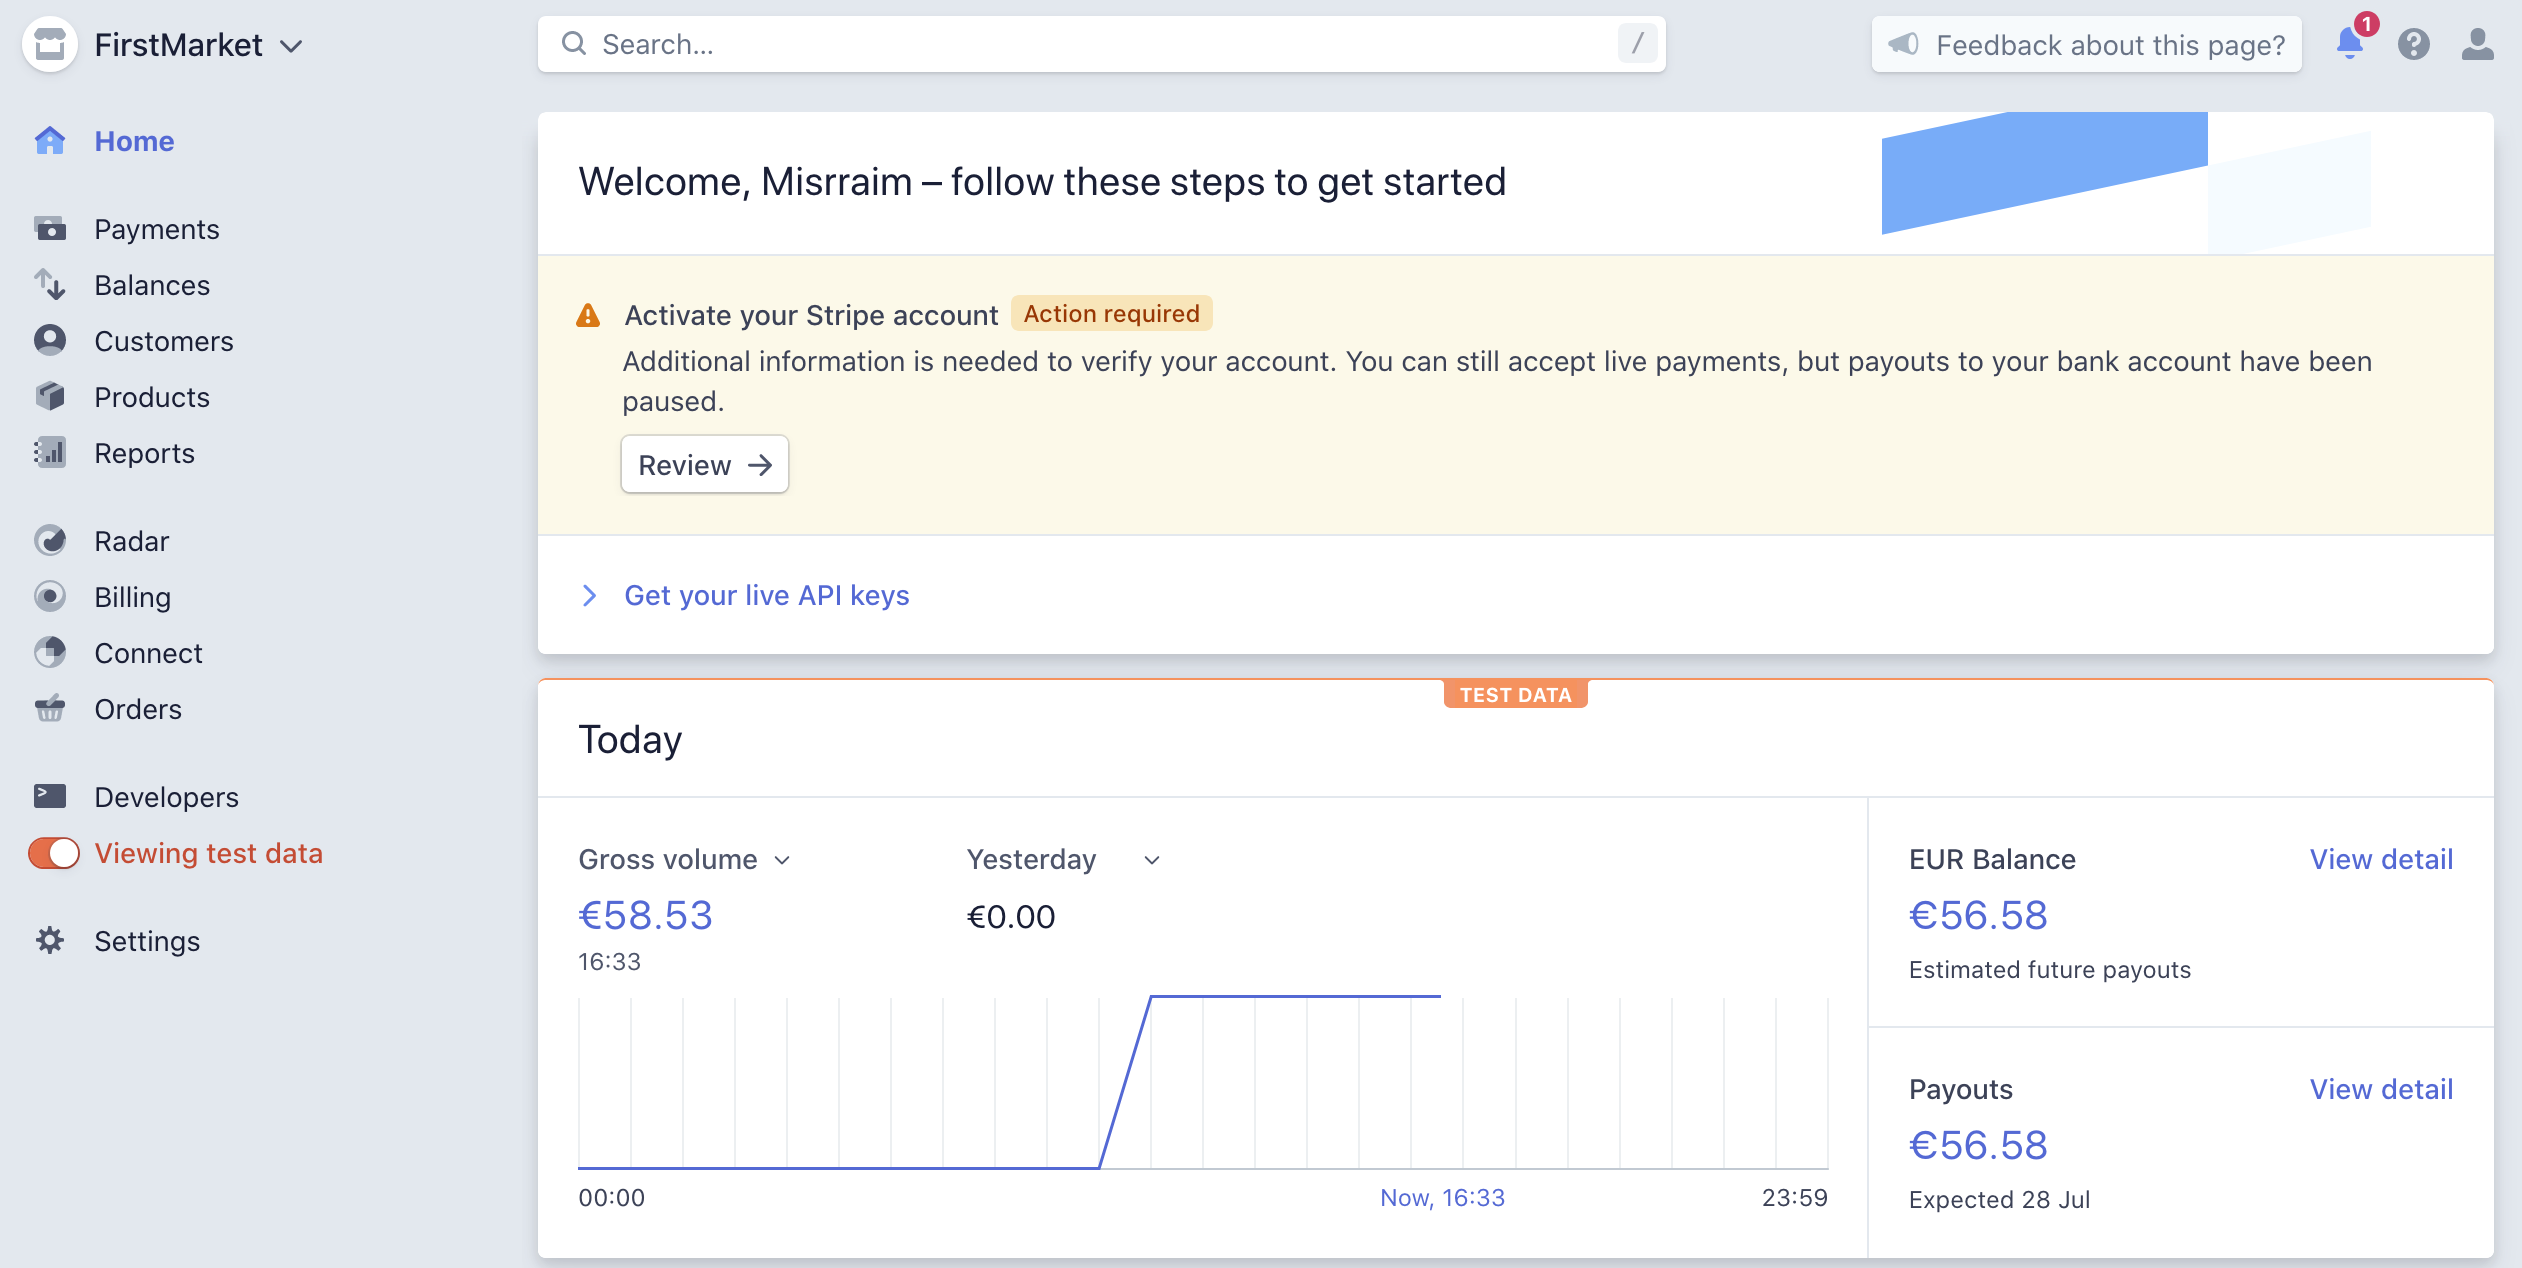
\includegraphics[width=\textwidth,keepaspectratio]{stripe_dashboard}
    	\caption{Stripe Dashboard}
    	\label{fig:stripe_dashboard}
    \end{figure}
    
    \paragraph{Stripe Radar}
    Como último apunte de esta sección dedicada a Stripe, destacar que esta herramientas de pago ofrece, sin coste añadido, su sistema anti-fraude \href{https://stripe.com/es/radar}{Stripe Radar}. Esta herramienta, basada en mecanismos de \href{https://stripe.com/es/radar/guide}{\emph{machine learning}}, asocia a cada transacción un índice de riesgo, tomando las acciones apropiadas en caso de que sea necesario (por ejemplo, si el riesgo fuese alto por defecto se bloquea la transacción). En la figura \ref{fig:stripe_radar} se muestra un ejemplo de evaluación de riesgo sobre una transacción.
    
    \begin{figure}[hbt!]
    	\centering
    	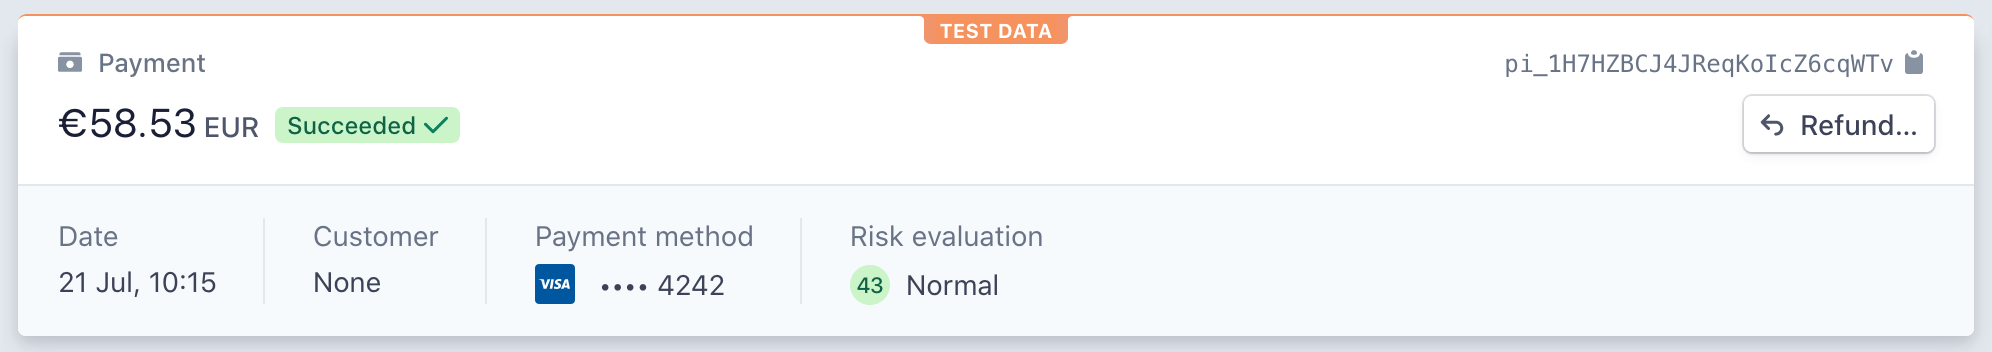
\includegraphics[width=\textwidth,keepaspectratio]{stripe_radar}
    	\caption{Evaluación del riesgo de una transacción con Stripe Radar}
    	\label{fig:stripe_radar}
    \end{figure}
    
    \section{Control de Concurrencia} \label{sec:concurrencia}
    Uno de los aspectos más críticos para el correcto funcionamiento de una tienda online es el control del stock de productos y del proceso de realización de una compra. Muchos usuarios, quizás simultáneamente, pueden añadir productos a sus cestas y proceder a su compra. La aplicación debe garantizar que estas acciones se realicen de forma a conservar en todo momento la consistencia de los datos.
    
    \begin{figure}[hbt!]
    	\centering
    	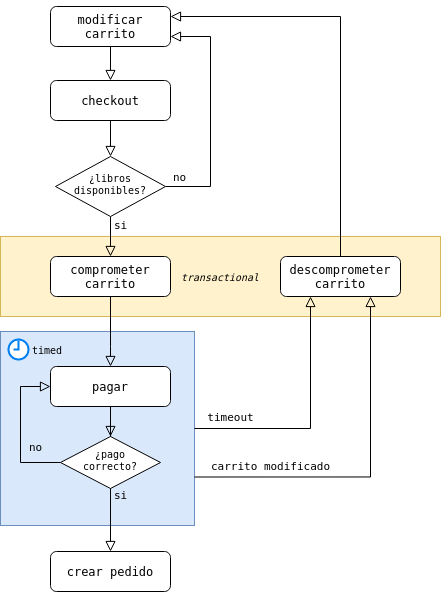
\includegraphics[width=0.7\textwidth,keepaspectratio]{cart_concurrent}
    	\caption{Diagrama del proceso de finalización de una compra}
    	\label{fig:cart_concurrent}
    \end{figure}
    
    Como se puede apreciar en la figura \ref{fig:cart_concurrent}, cuando un usuario decide proceder con el pedido de los libros contenidos en su cesta, lo primero que hace el sistema es comprobar que esos libros están disponibles. Pueden no estarlo por dos motivos, a saber, que estén agotados en ese momento o que el administrador de la aplicación web los haya deshabilitado (además, en este último caso el sistema automáticamente retira de la cesta dichos libros al detectar dicha situación). Si alguno de estos escenarios ocurriese la aplicación informaría al usuario en la propia vista de la cesta, sin avanzar a la vista de checkout, tal como se muestra en la figura \ref{fig:cart_alert}.
    
    \begin{figure}[hbt!]
    	\centering
    	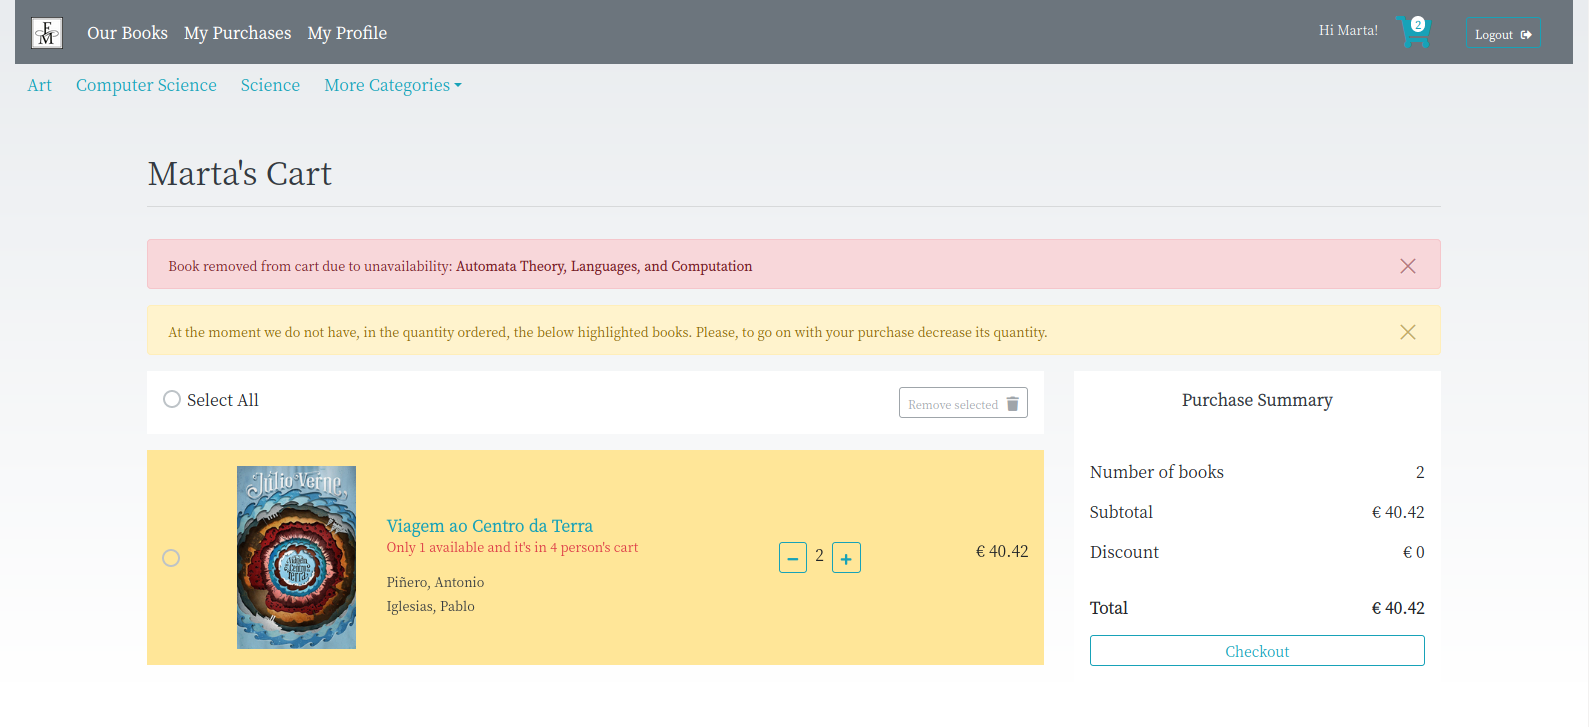
\includegraphics[width=\textwidth]{cart_alert}
    	\caption{Aviso por pantalla de no disponibilidad de libros}
    	\label{fig:cart_alert}
    \end{figure}
    
    Tras comprobar que los libros están disponibles el sistema \textbf{compromete} la cesta. Este es el paso fundamental donde se garantiza la consistencia. El sistema se compromete con el usuario a que si este finaliza la compra (dentro de un tiempo establecido) se le entregarán los libros seleccionados y al precio actual. Internamente, lo más destacado que el sistema realiza se recoge en:
    
    \begin{itemize}
    	\item[-] Se actualiza el stock, sustrayendo los libros en las cantidades correspondientes.
    	\item[-] Se crea en la base de datos una entidad \emph{sale} por cada item de la cesta, para así capturar el estado (principalmente el precio) de los libros en ese momento.
    	\item[-] Se contacta con Stripe para crear un nuevo \emph{Payment Intent}.
    	\item[-] Se activa el contador de tiempo disponible para finalizar la compra.
    \end{itemize}
    
    Todas estas acciones que realiza el sistema para comprometer la cesta las lleva a cabo de forma transaccional, apoyándose en la API de Spring Data JPA (ver \ref{sec:spring}). Las transacciones software se describen en términos de las características ACID, del acrónimo en inglés de Atomicity, Consistency, Isolation, y Durability:
    
    \begin{itemize}
    	\item[-] Atomicity. Cada paso en la secuencia de acciones realizadas dentro de los límites de una transacción deben completarse con éxito o todo el trabajo debe
    	retroceder. La finalización parcial no es posible, o sucede todo o no sucede nada.
    	\item[-] Consistency. Los recursos de un sistema deben estar en un estado coherente, no corrupto, tanto en el inicio como en la finalización de una transacción.
    	\item[-] Isolation. El resultado de una transacción no debe ser visible para otras transacciones hasta que la primera se confirme con éxito.
    	\item[-] Durability. El resultado de una transacción comprometida debe hacerse permanente, independientemente a cualquier fallo del sistema.
    \end{itemize}
    
    Una vez comprometida la cesta, que otro usuario modifique el stock (ya sea un cliente al comprar un libro o el administrador al variar el stock), o que el administrador varíe el precio de algún libro de los recién comprometidos, o que incluso deshabilite alguno de estos libros, sería transparente para el usuario que acaba de comprometer su cesta. Mientras dure el tiempo disponible para finalizar la compra, la cesta comprometida es un contrato inmodificable. En este punto pueden suceder dos cosas: 
    
    \begin{enumerate}
    	\item El usuario completa el formulario de checkout y paga correctamente dentro del plazo, en cuyo caso se tramitaría el nuevo pedido.
    	\item El tiempo disponible para finalizar el pago se agota sin haber sido realizado, o el usuario, en la vista de la cesta, modifica las cantidades de los libros. Ante ambos eventos el sistema procede a \textbf{descomprometer} la cesta, abortándose de facto la compra.
    \end{enumerate}
    
    El procedimiento de descomprometer la cesta es el inverso al de comprometerla, y también se realiza transaccionalmente. Así, lo más destacado que el sistema lleva a cabo internamente en este proceso se resume en:
    
    \begin{itemize}
    	\item[-] Se actualiza el stock, aumentando los libros en las cantidades correspondientes.
    	\item[-] Se eliminan las entidades \emph{sale} apropiadas de la base de datos.
    	\item[-] Se contacta con Stripe para cancelar el \emph{Payment Intent}.
    \end{itemize}

    \section[Datos Jerárquicos]{Persistencia y Visualización de Datos Jerárquicos} \label{sec:hierarchy}
    Desde muy pronto se reparó en la necesidad de gestionar en la base de datos información con relaciones de jerarquía, ya que las categorías de los libros están organizadas de esta manera. Además, si se implementase la funcionalidad de que los usuarios pudiesen añadir comentarios a los libros, con capacidad de respuestas anidadas, también se estaría en el escenario de estructuras jerárquicas.
    
    Tal como se explica con detalle en [bib ref], existen diversas formas de dar solución a esta necesidad, cada una de ellas con sus puntos fuertes y sus debilidades. La idoneidad de una solución frente a otra viene en gran medida determinada por la cantidad de información jerárquica a gestionar y por la frecuencia o importancia relativa de las operaciones de lectura, creación, actualización y eliminación.
    
    Si los datos jerárquicos son siempre de pequeño tamaño y las operaciones son principalmente de lectura, una solución sería cargarlos en memoria principal y gestionarlos desde allí con alguna estructura de datos apropiada. Este podría argumentarse que es el caso de la información de las categorías de los libros, ya que en principio estas no superarían a lo sumo algunas decenas de centenas, y la actividad principal realizada sería la lectura. La frecuencia con que el administrador de la tienda crea, modifica o elimina una categoría es despreciable respecto de la frecuencia con que las categorías son leídas por los usuarios en general.
    
    Por otro lado, si se implementase la funcionalidad de los comentarios anidados, el escenario es claramente diferente. La cantidad de información es potencialmente mucho mayor, con lo que trabajar directamente en memoria principal no es una opción. Además, las operaciones de creación, modificación y eliminación cobran mayor protagonismo.
    
    La solución más común en este caso se conoce como listas de adyacencia, y no es otra cosa que añadir a cada entidad una referencia (clave extranjera) al id de su predecesor jerárquico. El problema de esta solución es que escala muy mal a medida que aumenta la profundidad del árbol. Imagínese que se tiene un hilo de comentarios arbitrariamente profundo, el cual precisaría de consultas recurrentes por cada nivel si se pretendiera extraer todo el hilo (algo habitual en estos sistemas de comentarios), ya que a priori se desconoce la profundidad. Sin embargo, existen métodos para extraer todo el hilo de comentarios con una sola consulta (en general, extraer cualquier subárbol), como se verá a continuación.
    
    La funcionalidad de que los libros estén clasificados por categorías es imprescindible para la aplicación, y en consecuencia ha sido implementada. No es el caso de los comentarios. No obstante, en un intento de hacer la aplicación fácilmente ampliable en este sentido, y dado que se trata de un proyecto académico, se optó por una solución que fuese eficiente y versátil: la denominada \textbf{Closure Table}.
    
    La idea principal es mantener la información de las relaciones entre las entidades en una tabla diferente. Es decir, por una parte se encuentra la tabla \emph{category} y por otra la tabla \emph{catpath}. En la primera se almacena la información relativa a las categorías (su id, nombre, etc), mientras que en la segunda se almacena la información de los caminos en el árbol de categorías. De todos los caminos, incluso de una categoría consigo misma. Así, por cada fila en la tabla \emph{catpath} se tiene el identificador del ancestro (clave extranjera de la tabla \emph{category}), el identificador del descendiente (también clave extranjera de la tabla \emph{category}) y el tamaño del camino. Para una relación de una categoría consigo misma el tamaño del camino es 0, para una relación directa el tamaño es 1, abuelo-nieto es 2 y así sucesivamente.
    
    \begin{figure}[htb!]
    	\centering
    	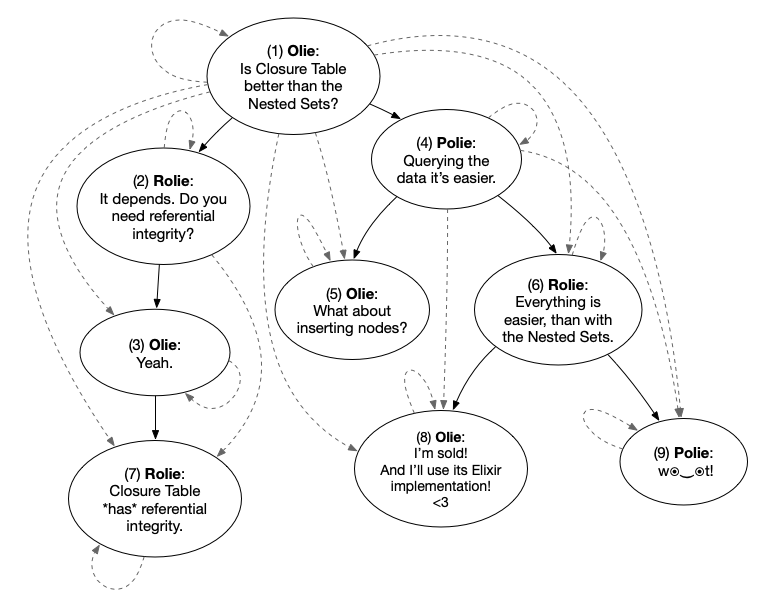
\includegraphics[width=0.7\textwidth]{closure_table}
    	\caption{Diagrama de conexiones registradas en una closure table}
    	\label{fig:closure_table}
    \end{figure}
    
    Esta solución es la más versátil y rápida de todas las mostradas en [bib ref], permitiendo incluso a un nodo pertenecer a varios árboles. Sin embargo, estos beneficios los consigue a costa de espacio. Este consumo puede ser importante si la estructura almacena jerarquías muy profundas.
    \\
    
    No obstante todo lo discutido con anterioridad, la solución real implementada para el trato específico de las categorías es triple (ver listado \ref{list:sql_cat}): Closure table, lista de adyacencia y trabajo en memoria principal con una estructura de datos en árbol. Esto es así por una cuestión de eficiencia y por desarrollar experiencia en el uso de estas soluciones.
    \\
    
    \begin{lstlisting}[caption=Tablas que gestionan las categorías,label=list:sql_cat]
    create table category (
    	id bigint not null, 
    	created_by varchar(255), 
    	created_date timestamp, 
    	last_modified_by varchar(255), 
    	last_modified_date timestamp, 
    	name varchar(255), 
    	parent_id bigint, 
    	primary key (id)
    );
    	
    create table catpath (
    	id bigint not null, 
    	created_by varchar(255), 
    	created_date timestamp, 
    	last_modified_by varchar(255), 
    	last_modified_date timestamp, 
    	size integer not null, 
    	ancestor_id bigint, 
    	descendant_id bigint, 
    	primary key (id)
    );
    
    alter table category 
    	add constraint fk_parentIdOnCategory foreign key (parent_id) references category(id)
    ;
    
    alter table catpath 
    	add constraint fk_ancestorIdOnCatpath foreign key (ancestor_id) references category(id)
    ;
    
    alter table catpath 
    	add constraint fk_descendantIdOnCatpath foreign key (descendant_id) references category(id)
    ;
    \end{lstlisting}
    
    Aparejado con el problema descrito en los párrafos anteriores se encuentra el de presentar al usuario dicha información jerárquica. Muy al principio del desarrollo de este proyecto se utilizó la tecnología de plantillas Java Server Pages para general el contenido HTML, la cual permite insertar en las vistas código Java de servidor. Así, se desarrolló una vista que contenía una función recursiva que permitía generar código HTML que mostrase la estructura anidada de las categorías. Pero esta aproximación de mezclar HTML y código Java de servidor es considerada una mala práctica y está en desuso.
    
    Posteriormente se adoptó el uso de Thymeleaf como motor de plantillas (ver \ref{sec:thymeleaf}), que no contempla esta posibilidad de insertar código de servidor en las vistas (al menos de la manera tan natural como lo permite JSP). Thymeleaf permite generar contenido lineal (una lista, por ejemplo) haciendo uso de la directiva \emph{th:each}, que hace las veces de bucle \emph{for}, pero para generar contenido anidado no dispone de ninguna funcionalidad nativa.
    
    Por todo lo anterior, para resolver este problema se optó por desarrollar código JavaScript (\emph{categoriesBuilder.js}) que se encargase, en el cliente, de construir y conectar, entre sí y al lugar apropiado en \emph{categories.html} (ver línea 15 del listado \ref{list:html_categories}), los componentes DOM necesarios para mostrar la estructura anidada de las categorías.
    \\
    
    \begin{lstlisting}[caption=Contenido principal de la vista categories.html,label=list:html_categories]
    <div class="container-fluid fm-content">
	    ...
	    <!-- main content -->
	    <div class="row">
		    <div class="col-sm-1"></div>
		    <div class="col-sm-10" id="root-hook">
			    <!-- new category -->
			    <div class="my-2 d-flex">
				    <a class="btn btn-outline-secondary align-center px-4 ml-auto" th:href="@{/admin/categoryForm}">
				    	<i class="fas fa-folder-plus fa-lg mr-4"></i>New Category
				    </a>
			    </div>
			    <hr/>
			    <!--
			    js dynamic generated content here
			    -->
		    </div>
		    <div class="col-sm-1"></div>
	    </div>
	    ...
    </div>
    \end{lstlisting}
    
    Como resultado, el administrador de la aplicación web puede visualizar la estructura jerárquica de las categorías a través de desplegables anidados, como se muestra en la figura \ref{fig:nested_categories}.
    
    \begin{figure}[htb!]
    	\centering
    	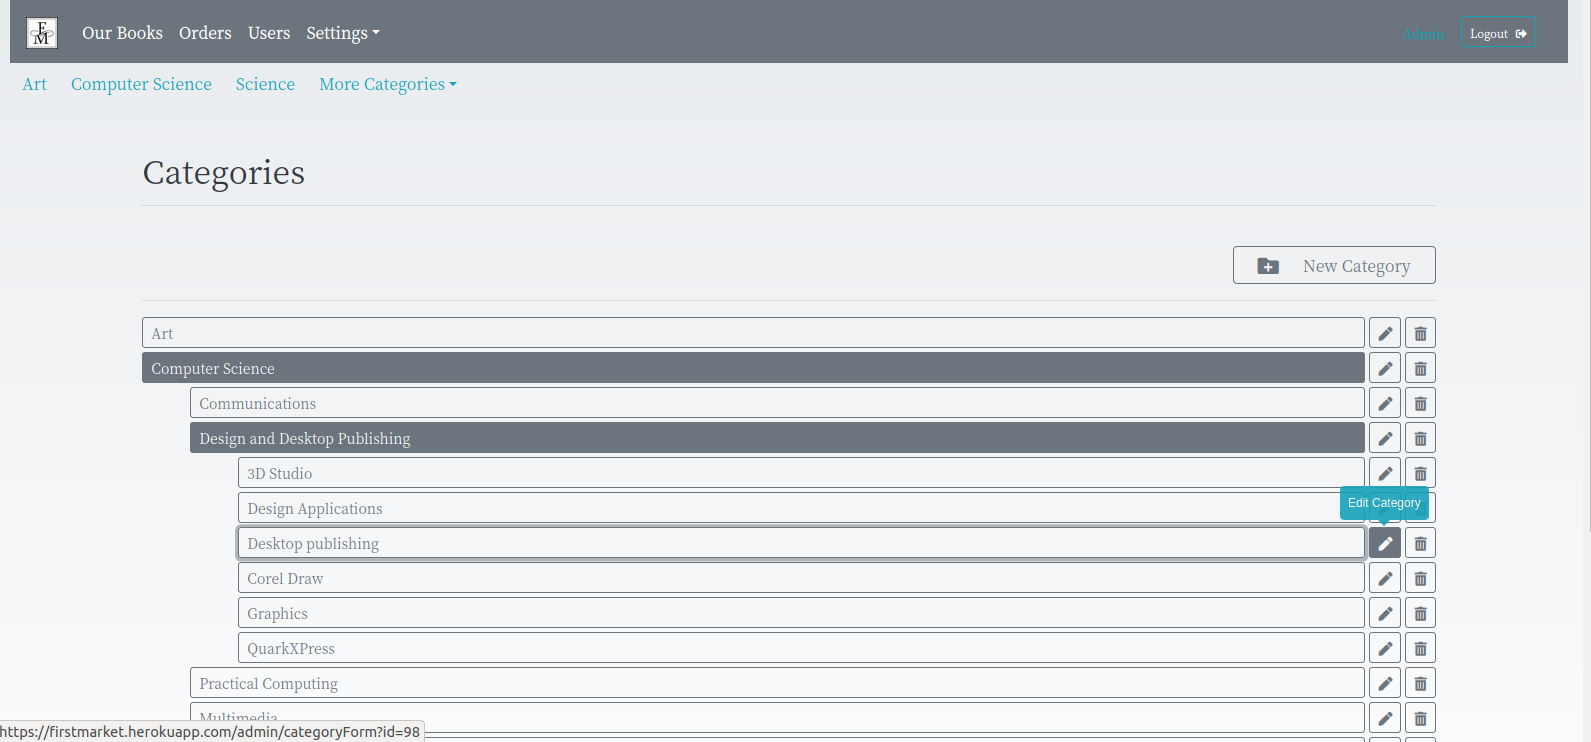
\includegraphics[width=\textwidth]{nested_categories}
    	\caption{Visualización de la estructura anidada de las categorías}
    	\label{fig:nested_categories}
    \end{figure}
    
    \section{Experiencia de Usuario Mejorada}
    Uno de los requisitos básicos de la aplicación web desarrollada es el de permitir a los usuarios gestionar su compra mediante el uso de una cesta virtual, que sirva de almacenamiento para la compra en curso. Esta funcionalidad permite a los usuarios:
    
    \begin{itemize}
    	\item[-] Añadir libros a la cesta. Esto se puede realizar desde cualquier vista que muestre información de un libro, a saber, la página de inicio, la página de resultados de búsqueda y la página de detalles de un libro.
    	\item[-] Modificar la cantidad de un libro en la cesta, o eliminar un libro de la cesta. Estas acciones se pueden realizar desde la vista de la cesta de un usuario.
    \end{itemize}
    
    Para la gestión de estas acciones, la arquitectura clásica de petición de un recurso por parte del cliente y respuesta con contenido HTML por parte del servidor (con su consecuente refresco de la página) se juzgó inapropiada. Un usuario que esté visualizando la página de su cesta y aumente en una unidad un libro tendría que esperar, para ver el resultado de dicho aumento, a que el servidor responda con el nuevo contenido HTML y que el navegador lo renderice, todo ello para únicamente cambiar unos pocos números respecto de la página previa. Situaciones similares ocurren en el caso de disminuir la cantidad de un libro, o eliminarlo de la cesta por completo. Peor aún es el caso del usuario que decide añadir un libro a su cesta, ya que el contenido HTML por el que debiera esperar sería igual (salvo el icono del número de elementos en la cesta) al de la página desde donde se solicita tal acción.
    
    En este contexto, y como pretexto perfecto para su estudio, se decidió desarrollar estas acciones con tecnología Ajax, de forma que no tenga lugar el refresco de la página en la que el usuario se encuentre. Así, el script \emph{ajaxCart.js} se encarga, entre otras cosas, de actualizar el DOM de la vista de la cesta del usuario, \emph{cart.html}, de manera consistente con las acciones que este realice, mientras que el script \emph{ajaxAddBook.js} gestiona el DOM de las citadas vistas desde las cuales es posible añadir libros a la cesta. Ambos scripts establecen en background la comunicación con el servidor, de forma transparente al usuario, haciendo uso del objeto \emph{XMLHttpRequest}, tal como muestra el extracto de \emph{ajaxCart.js} mostrado en el listado \ref{list:js_ajax}.
    \\
    
    \begin{lstlisting}[language=JavaScript,caption=Comunicación Ajax con el servidor,label=list:js_ajax]
    xmlHttpRequest = new XMLHttpRequest();
    xmlHttpRequest.open("GET", url, true);
    xmlHttpRequest.setRequestHeader('isAjaxCartRequested', '1');
    xmlHttpRequest.send();
    xmlHttpRequest.onreadystatechange = function() {
    	if (this.readyState === 4 && this.status === 200) {
    		onHttpOk(action, id, this.responseText);
    	}
    	if (this.readyState === 4 && this.status === 401) {
    		onHttpUnauthorized();
    	}
    };
    \end{lstlisting}
    
    \section[Libros Referenciados ]{Registro de Libros Referenciados en Cestas}
    En este apartado se describe una funcionalidad añadida que, si bien no estaba presente en los requisitos de la aplicación, se ha mostrado muy útil y de relativa facilidad de implementación. La inspiración provino, como se aprecia en la figura \ref{fig:etsy}, del portal de comercio electrónico \href{https://www.etsy.com}{Etsy}, al querer imitar su capacidad de informar de la situación en la que, para un producto determinado, queden igual o menos unidades en stock de las que están siendo referenciadas en cestas de los usuarios. Esto es, que un libro esté en la cesta de \emph{x} usuarios diferentes, que de ese mismo libro queden en stock \emph{y} unidades, y que \emph{x} sea igual o mayor que \emph{y}.
    
    \begin{figure}[htb!]
    	\centering
    	
\includegraphics[width=0.5\textwidth]{etsy}
    	\caption{Aviso de producto escaso y demandado en Etsy.com}
    	\label{fig:etsy}
    \end{figure}
    
    Con este objetivo en mente, se pensó en tres alternativas para implementarlo. Por un lado, la solución trivial sería realizar una consulta a la base de datos para conocer de esta situación cada vez que se necesite mostrar al usuario información de un libro. En este sentido, sería necesario explorar las cestas de todos los usuarios, para cada libro del cual se requiera información. No es desacertado estimar que la frecuencia con se requiere información de libros en una tienda de libros sea alta. Además, el número de usuarios puede ser todo lo grande que se pueda. Por ello, esta solución sería bastante pobre en tiempo de respuesta.
    
    La segunda alternativa, con objeto a disminuir el tiempo de respuesta, sería aumentar la información de cada libro que se almacena en la base de datos, creando un nuevo campo en el que se contabilizase el número de referencias que a dicho libro le son realizadas en las cestas de los usuarios. Esta solución sería muy rápida, pero a costa de un uso redundante de los recursos de almacenamiento, puesto que la información necesaria \emph{ya} estaba en la base de datos.
    
    Finalmente, la tercera vía, que es la implementada, trata de aunar rapidez y no redundancia en la base de datos. Esto se consigue manteniendo la información necesaria en una estructura de datos llave-valor en memoria principal, sólo para los libros referenciados. La llave sería el \emph{id} de un libro, y el valor el número de referencias en cestas que posea. Los tiempos necesarios para consultar esta estructura de datos, así como para actualizarla, son muy bajos. Además, la base de datos se mantiene no redundante. Es cierto que existe un grado de redundancia, pero esta es ajena a la base de datos, y se limita a los libros que estén referenciados (en contraste con la segunda solución, en la que \emph{todos} los libros en la base de datos ampliaban su información).
    
    Esta estructura de datos es mantenida eficientemente por la clase \emph{BookServer}, como se aprecia en el listado \ref{list:java_cartbooks}, de manera que cada vez que algún usuario añade o elimina un libro de su cesta queda reflejado en el registro.
    \\
    
    \begin{lstlisting}[language=Java,caption=Gestión del registro de libros referenciados en cestas,label=list:java_cartbooks]
    @Service
    public class BookServer {
    
    	private final Map<Long,Integer> cartBookRegistry = new HashMap<>();
    	
    	...
    	
	    public void incrementCartBookRegistry(Long cartBookId) {
		    cartBookRegistry.merge(cartBookId, 1, (oldValue, defaultValue) -> ++oldValue);
	    }
	    
	    public void decrementCartBookRegistry(Long cartBookId) {
		    cartBookRegistry.computeIfPresent(cartBookId, (key, value) -> (value > 1L) ? --value : null);
	    }
	    
	    public void incrementCartBookRegistry(List<Long> cartBookIds) {
	    	cartBookIds.forEach(this::incrementCartBookRegistry);
	    }
	    
	    public Map<Long,Integer> getCartBookRegistry() {
	    	return cartBookRegistry;
	    }
    }
    \end{lstlisting}
    
    Así, este registro es utilizado para avisar a los usuarios cuando un libro presenta escasez y alta demanda, como se muestra en la figura \ref{fig:fm_cartBookRegistry_alert}. Pero también es usado como \textbf{medida de la popularidad} de los libros, empleándose este uso en la página de inicio de la aplicación. Es cierto que el parámetro \emph{popularidad} se puede definir de muchas maneras, y que sería conveniente que en él se reflejase el volumen de ventas en una ventana temporal local, pero como una primera aproximación de bajo coste al concepto funciona perfectamente.
    
    \begin{figure}[htb!]
    	\centering
    	
\includegraphics[width=\textwidth]{fm_cartBookRegistry_alert}
    	\caption{Aviso de producto escaso y demandado en FirstMarket}
    	\label{fig:fm_cartBookRegistry_alert}
    \end{figure}